%*****************************************************************************************
%*********************************** First Chapter ***************************************
%*****************************************************************************************

\chapter{Introduction}  %Title of the First Chapter

% **************************** Define Graphics Path **************************
\graphicspath{{Chapter1/Figs/}{Chapter1/Figs/}}

\vspace{1mm}
\footnotesize {
\begin{flushright}
\textit{
Let us try teaching children \textbf{how to think} instead of what to think.
}\\
\end{flushright}
}
\vspace{1mm}


%-----------------------------------------------------------------------------------
\section{What is {\librER}?}
%-----------------------------------------------------------------------------------
{\librER} is inspired by KHAN academy \cite{KHAN} which is a non-profit organization
with the goal of changing education for the better. In the same fashion, {\librER} 
has also been thought to be a non-profit organization in which the main goals are 
fivefold:
\begin{itemize}[noitemsep,topsep=0pt,parsep=0pt,partopsep=0pt]
 \item to contribute to the development of a free world-class education in Robotics 
 for anyone anywhere;
 \item to design and build low-cost robots with high standards of quality;
 \item to improve current open source software projects so as to be more approachable 
 by inexperienced users; 
 \item to design free access material in educational Robotics, and develop activities 
 where organization and cooperation of the participants can foster
 possible solutions for environmental, social and healthcare issues; and
 \item to design and build environments where participants can discover and
 develop their own capabilities.
\end{itemize}

{\librER} will provide software and hardware for educational robots that are extremely 
reliable (robust), modifiable, and very cheap in order to be accessible to anyone and 
to enable a much more rapid development of the community.

In addition to that, {\librER} has been adopted the philosophy of free software 
foundation, since free and open-source software and hardware licences state that anyone 
is freely licensed to use, copy, study and change in any way, and the source code is 
openly shared so that users are encouraged to voluntarily improve the design of the 
software. As Meyer \cite{Meyer2003} put it,``Libre software offers scientists the 
possibility of sharing with their peers how they have solved problems. This, of course 
is basic for the evolution of science; but libre software goes beyond tha and makes 
this happen in a cost-effective way.'' 

%-----------------------------------------------------------------------------------
\section{What are the Benefits for Learning and Sharing with {\librER}?}
%-----------------------------------------------------------------------------------
There are many benefits that can be derived from {\librER}, mainly because the 
creation of strong links between industry, government, education and sociecity. 
Robotics is a multidisiplinary field in which mathematics, physicis, mechanics, 
computational science and electronics to mention but a few are applied.
Robotics applications have been proven to be many and these are ranging from 
agriculture to factory automation, from healthcare to education \cite{ashesirobotics2013}. 
Aditionally, robotics is a fascinating and fun way to develop creativity as well as the 
design, implementation, and integration of ideas that are essential for the development 
of skills that provides participants to cooperate and build conditions for a better world. 
Henceforth, similar projects of educational robotics that epitomise benefits for their 
communities are reviewed in the following section.

Valeria Larrar, a primary professor from Argentine, designed various workshops in educational 
robotics for participants between 10 and 15 years old in public schools. Valeria at a TED 
talk \cite{Larrart2013} in October 2013 mentioned that having seen the succefulness and 
possibilities of his first workshop, the educational ministery of Argentine afforded her 
school to buy 30 Robotics LEGO kits. It is important to mention that one of the goals 
for workshops is to tackle common issues in the community, for example, having known 
the problem of usefulness of traffic lights in busy highways, students built an 
automatized bridge to transport mainly disable people. Valeria emphasised that the power 
of interest is really great that what it looks like a professor guiding his pupils 
(Figure \ref{fig:educationalroboticsprojects}), in reality that person is the school 
caretaker who is delighted by the educational robotics software.
\begin{figure}[htbp!] 
\centering    
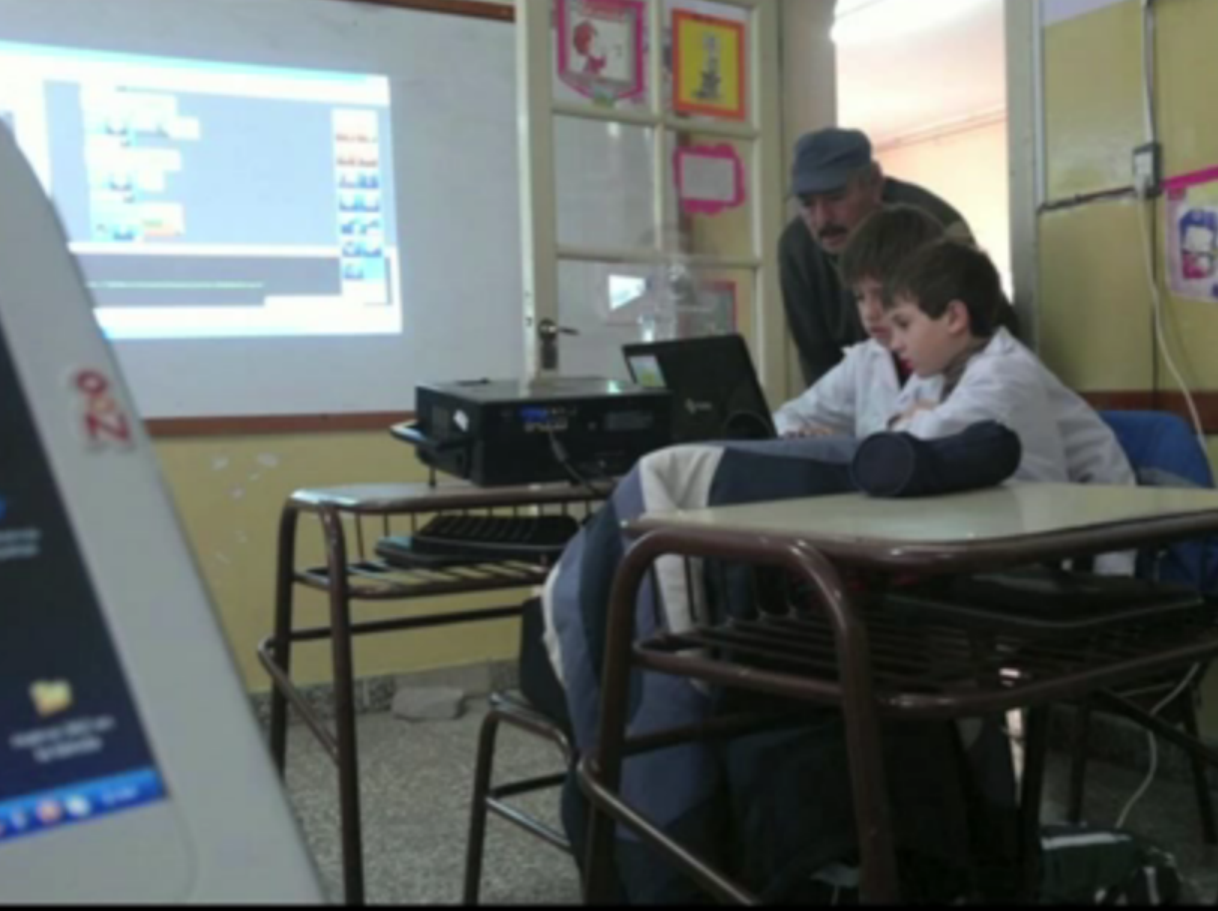
\includegraphics[width=0.4\textwidth]{chicos_and_conserge.png}
\caption[PA]{A school caretaker watching the boys using educational robotics software.}
\label{fig:educationalroboticsprojects}
\end{figure}
Valeria's projects showed that by learning robotics, students can create many 
oportunities, relationships among parents and sibilings, friends, and most importantly
finding joyness and optimismn in doing something that they love.

Similarly, the Ashesi Robotics Experience (ARX), an annual robotics workshop in Africa,
is designed to provide a stimulating, fun and refreshing environment 
for students to learn robotics \cite{ARX2013}. At ARX 2013 mentors were selected
from Ashesi University College who possessed the right set of skills and attributes 
to mentor, train, and take responsability of students. During one week, students 
were working on building Lollybots and LEGO Mindstorm Robots and 
on the last day, the community where invited to see students' projects 
so as to show that Robotics can be used as a way of critical thinking to solve social 
problems.
ARX also provides statistics of the participants in which the number of boys were 34, 
representing 57\% of participants, while girls were 26, representing the other 43\%. 
Participants were between the ages of 15 to 21 and came from all nine regions of Ghana, 
as well as two international students from Ethiopia and Swaziland 
(Figure \ref{fig:arx2013}).
\begin{figure}[htbp!] 
\centering    
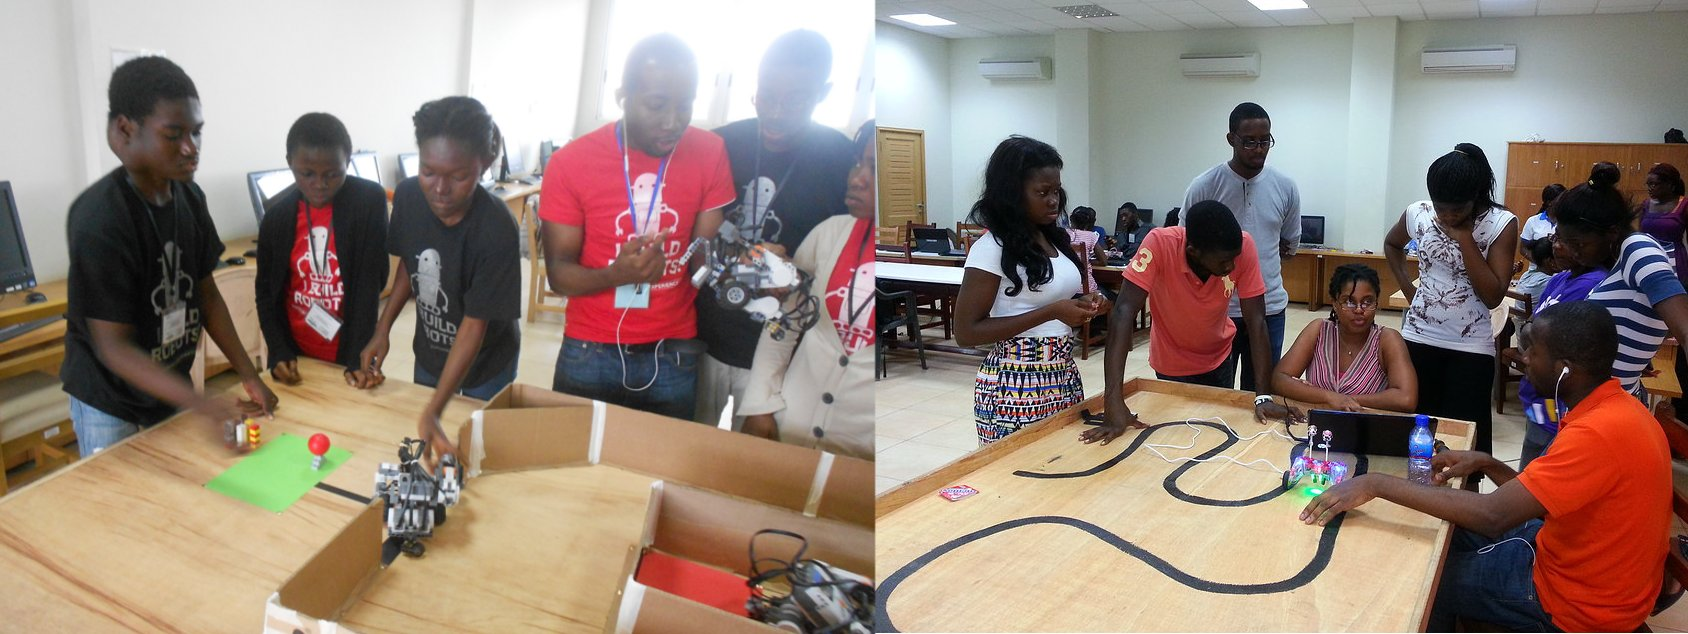
\includegraphics[width=0.75\textwidth]{arx2013_main.jpg}
\caption[PA]{Ashesi Robotics Experience Workshop 2013}
\label{fig:arx2013}
\end{figure}
Additionally, Ashesi Robotics posted several final projects at their webpage 
\cite{ashesirobotics2013}, for instance, exploration robots,
Planning in Dynamic Environment, Building a Sorter Robot, Follow the leader,
Tic-tac-toe, Dynamic balancing and Robot Navigation using colors as road signs.
It is important to note that all projects were documented by using 
these outline: Introduction, Approach, Algorithm, Results, Conclusion, and Appendix.

Having checked the positive benefits, one can see that many of the previos-mentioned 
projects were implemented with LEGO Mindstorm Robots which represent a signigicantly 
economical inversion. To this end, The African Robotics Network (AFRON) 
community presented a project called ``Ultra Affordable Educational Robot'' in 
which many participants around the world are called to present their robot designs 
that can inspire young children worldwide about Science, Technology, Engineering, 
and Math \cite{AFRON2014}. One of the primary goals for Ultra Affordable Educational 
Robot is to make robots that are more functional, more realiable, easier to use, less 
expensive and easier to manufacture. At the AFRON Design Challenge 3 categories were
considered: 
1) hardware 2) software, or 3) curriculum (Figure \ref{fig:afron2014}). First places 
are going to be cited, however, second and third places are worth of reviewing in the 
future. Both in the hardware and curriculum categories, The MIT SEG: An Origami-Inspired 
Segway Robot won the first place mainly because of  its accesible price of 
approximately \$20 US dollars 
\cite{MITPrintableRobot2013}. MIT SEG's software is based on ardublock
\cite{Ardublock2013}  for which activities were taught using finite state machine 
concepts. In the software category, AERobot: an Affordable Education Robot won the first 
place \cite{AERobot2013}. AERobot's software is based on Minibloqs, a graphical 
programming environment \cite{minibloq2011}, that allow novice programmers to easily 
program their little Robot.
\begin{figure}[htbp!] 
\centering    
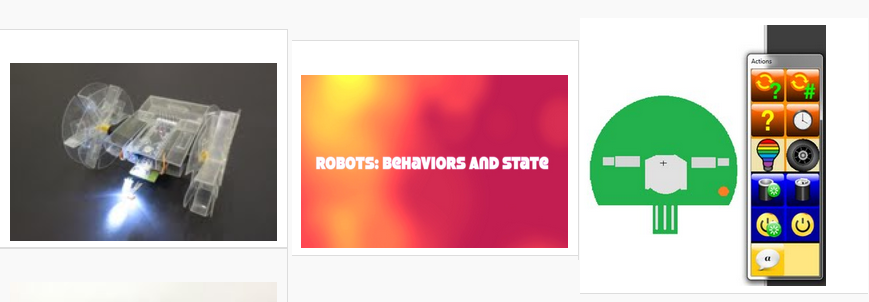
\includegraphics[width=0.8\textwidth]{afron2014}
\caption[PA]{First places at the AFRON Design Challenge: The MIT SEG, Behaviors and 
states with finite state machine concepts, and  AERobot's software based on minibloq
(from left to right).}
\label{fig:afron2014}
\end{figure}

It is also important to note that there are many related projects for educational robots, 
that are not open source software and hardware projects with high prices that are out 
of the current economical posibilities, for instance, Finch Robot \cite{finchrobot2014} 
and Bee-Bot \cite{bee-bot2014}; however, both provide a good references for lessons 
and software tools.
